\chapter{Arbejdsmetoder}\label{kapitel_Arbejdsmetoder}
Under projektarbejdet har gruppen benyttet sig af en række arbejdsmetoder til styring og udvikling.
Her beskrives disse metoder samt en opremsning af de udviklingsværktøjer, gruppen har benyttet.

\section{Projektstyring}
Alle gruppens medlemmer har i starten af udviklingen underskrevet en samarbejdsaftale (se bilag nr. XX). Denne sikrer enighed omkring udviklingen og definering af kravene. \\
\newline
Der er ved projektets begyndelse udarbejdet en tidsplan til overblik og gennemførsel af projektforløbet. Denne er udviklet efter ASE-modellen, men efter en agil tankegang, hvor tidsplanen kan skydes i forhold til hvilke ændringer og krav der kommer. (???). Tidsplanen bruges til styring af projektet, således at slutproduktet nås i tid til at kunne lave en fuldbyrdig accepttest og for at sikre afleveringsdatoen. \\

\begin{figure}[H]
\centering
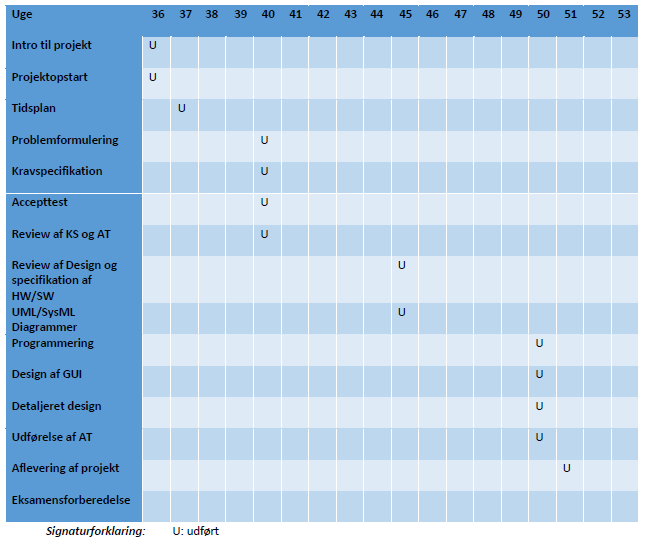
\includegraphics[scale=0.70]{tidsplan.PNG}
\caption{Tidsplan}
\end{figure}

\subsubsection{Scrum}
Projektets udførsel er inspireret af Scrum.\\
Brugen af Scrum ses i Pivotal Tracker (PT), hvor alle delopgaverne angives som sprints og gruppens medlemmer, enten individuelt eller i mindre enheder, kan "starte"\ en opgave, og "afslutte"\ når denne er færdig. Delopgaverne er i hovedtræk angivet med deadlines i tidsplanen, og er i PT prioriteret og markeret med opgavens størrelse fra 1-5. For at kunne følge med i udviklingen og se tilbage på hvilke gruppemedlemmer der udviklede hvilke delopgaver, er der tilføjet en eller flere ansvarlige for delopgaverne. 

Der er, fra starten af projektets udførsel, taget udgangspunkt i Scrum som arbejdsværktøj. 
Scrum er valgt som framework, fordi en lang række af metoderne, herunder den empiriske proces, har været anvendelige i forhold til projektet. Dette giver en god stuktur og gør det nemmere at holde overblikket undervejs i projektet.\\
Ved valg af Scrum som framework blev der sat nogle krav til hvilke roller, artefakter, regler og møder, der skulle være til stede for, at det fungerede. \\
I projektet er der kun anvendt dele af Scrum, da der ikke har været mulighed for at have en Scrum Master og kun en tilnærmelsesvis Product Owner.\\
Der er ligeledes indgået kompromisser omkring andre regler inden for Scrum, for at det har givet mening at anvende Scrum som værktøj i projektet.\\
\newline
Scrum Teamet i projektet har bestået af vejlederen som Product Owner, projektgruppen som Development Team og reelt set ingen Scrum Master. \\
Igennem dokumentet ”Vejledning til 3. semesterprojekt”\ er Product Backloggen defineret af vejlederne, og har derfor dannet grobund for udviklingen af projektet fra begyndelsen.\\ 
Product Backloggen har dog ikke været fuldstændig fastlagt i og med, at Development Teamet skulle forstille sig et scenarie, hvori produktet kunne anvendes. Scenariet hvor blodtryksmåleren skal figurere i, er i dette projekt, valgt til en operationsstue på et hospital. Ud fra dette scenarie er der blevet taget stilling til hvilke funktionaliteter, der var nødvendige og skulle tilføjes til Produckt Backloggen. Et eksempel er overvejelsen omkring en ”akut knap”, som ville springe nogle formelle procedure over i tilfælde af en akut situation, men denne er fravalgt efter nærmere undersøgelse af kravene der stilles i scenariet ude på dagkirugisk afsnit.\\
\newline
Development Teamet blev fra start delt op i to mindre teams i HW og SW, både for at effektivisere arbejdet, og fordi det rent praktisk ikke har været muligt for alle at være til stede til det Daily Scrum møde. Der er altså dannet en form for sub-teams, selv om dette ikke oprindeligt er tilladt i Scrum, hvorfor møderne i forhold til Daily Scrum hovedsagligt forgået i de to mindre grupper. \\
Den overordnede tidsplan for projektet blev fastlagt forinden projektets begyndelse af Development Teamet, med udgangspunkt i de deadlines der i forvejen var fastlagt af vejlederne. Der var altså i alt 4 sprints hvor der cirka har været en måned til hver: 1. deadline var kravspecifikation, 2. Design og specifikationer af hardware og software, 3. Accepttest og 4. Projektaflevering.
Til hver af de fire Sprints er der blevet lavet Sprint Planning Meeting Sprint Backlog i takt med et nyt Sprint skulle påbegyndes.
Sprint Planning Meeting har fungeret som mødet, hvor begge Developments Teams var til stede og der blev fastlagt en overordnet Sprint Backlog. Her var der fokus på, hvad der skulle leveres i det pågældende Sprint, og hvordan der skulle arbejdes for at opnå dette.\\ Efterfølgende blev Sprint Backloggen ydereligere udspecificeret i de to Teams med henblik på deres fokusområder. Her var Projekt Owneren til dels også inde over i situationer, hvor der var tvivl om Product Backlog items.\\
Til at lave en Sprint Backlog har der i projektet været anvendt Privotal Tracker, som er en online Scrum tjeneste. Her har det været nemt og overskueligt at danne sig et overblik over, hvilke opgave der var i gangsat, hvilken udvikler der har påtaget sig opgaven, samt hvad der mangler at blive lavet.
Privotal Tracker tilbyder også at tilføje artefakter og dermed give en vurdering af opgavens værdi. Denne funktion er blevet fravalgt i projektet i og med, at der ikke har været tilstrækkelig erfaring omkring projektets emner til at lave en sådan vurdering.
Tilsvarende er orden heller ikke blevet brugt i så høj grad på Privotal Tracker, men kun i mundlig form i sammenhæng med diverse møder. \\
\newline
Hvert Sprint blev der fulgt op på ved hjælp af reviews med en anden gruppe. Her er der blevet lavet en vurdering af inkrementet og foretaget eventuelle ændringer til Product Backloggen, som skulle færdiggøres inden påbegyndelsen af næste Sprint. \\
\newline        
Der har været en relativ god forståelse af Scrum og dets arbejdsmetoder forinden beslutningen om at anvende det i projektet, men der er lang vej til, at det kunne have været gennemført fuldt ud. \\
Manglen på en Scrum Master som har kunnet styre Develpments Teams og sørge for opretholde Scrums regelsæt har været en klar mangel. 
Der har i mindre grad også været mangel på en Produkt Owner, men det har dog været nemmere at se bort fra, da der har været en klar Product Backlog fra start. Produkt Owneren har i projektet været flere personer i form af vejlederne, og dermed er der ikke overholdt Scrum’s regelsæt. Dette har medført, at det har været svært at finde ud af, hvem der skulle kontaktes ved ændringer undervejs i Product Backloggen. Ændringerne er altså blevet foretaget ved direkte kontakt fra Develeopment Teamet til Produkt Owner uden en Scrum Master til at styre det. 

\section{Udviklingsproces}
Projektets udviklingsproces er inspireret af agile metoder, som er en fleksibel og tilpasningsdygtig metode. Projektet foretages i små sprints, hvilket kræver meget kommunikation gruppen imellem. Den agile udviklingsproces giver en fleksibilietet i forhold til ændringer der kommer i løbet af gennemførelsen, hvilket har været nødvendigt i projektet, specielt i software-udviklingen.\\
\newline
Mere specifikt er projektet udviklet vha. den agile ASE proces. ASE-modellen er en semi-iterativ udviklingsproces, som drives af UC's, specificeret i kravspecifikationen i startfasen af projektet. ASE-modellen er inspireret af vandfaldsmodellen, hvor projektet ligeledes inddeles i faser, udvikles step for step og testes, og V-modellen, hvor der testes efter hver fase, og det derfor er nemmere at finde eventuelle fejl i løbet af udviklingen.\\
\newline
Vandfaldsmodellen er specifikt brugt i starten af projektets udvikling, hvor denne inddeles i steps. Disse steps blev udviklets af gruppen som samlet enhed, og indebærer bl.a. problemformulering, UC's, krav, accepttest og tidsplan. Efter denne specifikation af projektet, er gruppen delt op i to, en hardware- og en softwaregruppe.

\begin{figure}[H]
\centering
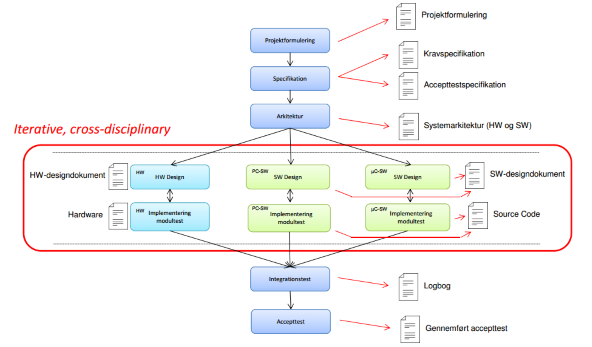
\includegraphics[scale=0.80]{ase.PNG}
\caption{ASE-modellen}
\end{figure}

V-modellen er brugt i test af software, i hht. integrationstest og modultests og en accepttest for kunden (gruppens vejleder) af hele systemet. \\
\newline
For at sikre at ingen af projektets dokumenter mistes, er delingsværktøjet Github anvendt. Her gemmes dokumenterne i en individuel mappe på hver af gruppemedlemmernes computere samt i "skyen". Github gemmer en versionshistorik af ændringer i dokumenterne, som angives heri.  

\section{Udviklingsværktøjer} %*Hed før redskaber
I udviklingen og implementeringen af projektet, er følgende udviklingsværktøjer anvendt:
\subsubsection{DAQ:}
USB-device fra National Instrument. Bruges til at opsamle data som vha. konvertering danner et digitalt signal.
\subsubsection{Analog Discovery:}
Generer et analogt signal ud fra blodtryksdata. Dette analoge signal konverteres, vha. DAQ'en, til et digitalt signal.
\subsubsection{WaveForms:}
Bruges sammen med Analog Discovery og DAQ'en til at indsende data til programmet (???)
\subsubsection{Visual Studio:}
Visual studio er et udviklingsværktøj til software. Dette program er anvendt til at designe software-delen. Programmeringssproget, der er anvendt her, er C$\#$. 
\subsubsection{Microsoft Visio:}
Microsoftprogram til udvikling af hardware-/software diagrammer. Anvendes til at forenkle komplekse oplysninger via enkle, letforståelige diagrammer.
\subsubsection{Multisim:}
Til design af hardware komponeneter til forstærkeren er simuleringsværktøjet Multisim anvendt. 
\subsubsection{Ultiboard:}
Til udlægning af print er programmet Ultiboard benyttet. Det er godt integreret med Multisim, og var derfor det oplagte valg.
\subsubsection{Github:}
Github er et delingsværktøj, som automatisk opretter et versionshistorik. Denne er derfor anvendt til dokumentdeling igennem projektet. 
\subsubsection{Pivotal Tracker:}
Pivotal tracker er anvendt som scrumboard til at styre projektets løbende arbejdsopgaver. 
\subsubsection{Mathad:}
Matchad er et regneværktøj, som er anvendt til at udføre beregner i Hardware-delen. 
\subsubsection{Latex:}
Latex er et såkaldt opmærkningssprog, som er velegnet til rapportskrivning, derfor er dette valgt til projektrapporten. 

\section{Rollefordeling}
\subsubsection{Mødestruktur}
Gruppen har ved projektets start, i samarbejde med vejlederen, fastlagt den overordnede mødestruktur. Projektgruppen er i udviklingen af hardware og software inddelt i to undergrupper - en hardwaregruppe og en softwaregruppe. Der er fastlagt et ugentligt møde med vejleder, planlagt efter hvordan ugen forløber, og mindst et ugentligt møde HW- og SW grupperne imellem. Møder  undergrupperne imellem, fastlægges efter behov, men også mindst én gang ugentligt. I perioder har dette været et møde i ugen, andre gange 4-5 møder i ugen. Kravene til møderne er defineret i samarbejdskontrakten (bilag XX). \\
\newline
Møder med vejleder er aftalt over mail fra gang til gang, hvor også en dagsorden er sendt med. Denne danner grundlag om mødet og sikrer, at alle punkter gennemgåes. Møder gruppen imellem aftales efter hvert enkelt møde, hvor der også her har været udviklet en dagsorden - dog kun til de møder, hvor denne har givet mening.\\
\newline
Der er lavet mødereferater for samtlige møder med vejleder og for reviews med andre projektgrupper. Derudover er der lavet logbøger ved samtlige møder gruppemedlemmerne imellem, både samlet og i undergrupperne. Mødereferaterne og logbøgerne sikrer at beslutningerne, taget ved de forskellige møder, altid kan refereres tilbage, hvorfor der ikke opstår tvivl om hvorvidt beslutningen blev taget, af hvem og hvad der overordnet blev argumenteret for.\\
Mødereferater og logbøger er skrevet i hvert sit dokument i Latex (bilag XX), hvor de hver især er angivet med mødenummer, dato, referent og tilstedeværende gruppemedlemmer.  

\subsubsection{Deadlines}
Der har fra projektets start været deadlines til dele af projektet. Disse har af overordnet karakter været angivet fra IHA's side, hvor gruppen, ud fra tidsplanen, har angivet flere og mere detaljerede deadlines for at sikre stabil fremgang i projektets gennemførsel. \\
Den første, og yderst væsentlige, deadline bestod af kravpecifikation og accepttest, som det også ses i tidsplanen (bilag X). Disse dokumenter udvikles af projektgruppen som samlet enhed, hvor gruppen arbejde i fællesskab om at definere projektets krav i hht. løsningen af problemet. Kravspecifikation og accepttest udvikles parallelt, i og med at disse skal stemme fuldstændig overens. \\
\newline
Ligeledes har der været deadlines i forhold til design og implementering, som bruges til design og beskrivelse af projektet.\\
\newline
Den sidste overordnede deadline består af accepttest, hvor hele systemet testes i hht. projektets definerede krav. Dette gøres sammen med kunden, som i dette tilfælde er vejlederen. 

%SKAL DER FLERE DEADLINES IND? 

\subsubsection{Review}
I følgeskab med de fra IHA's side angivede deadlines, var der krav om review. Dette indebar review af kravspecifikation og accepttest samt af arkitekturdesign. Et review er en session, hvor en anden gruppe læser det akutelle dokument igennem, hvorfor der kommer et objektivt syn på dokumentet. Review-gruppens kommentarer diskuteres til der opnås enighed omkring forståelsen af rettelserne, og dokumentindehaverne kan dermed tilrette dokumenterne i det omfang gruppen synes relevant. Der blev holdt review med to forskellige projektgrupper i forbindelse med de forskellige dokumenter, for at bibeholde det objektive syn på dokumentet. Dette objektive syn og den konstruktive kritik et review ofte resulterer i, er yderst nyttigt for projektets videre arbejde og sikrer at den ønskede forståelse af dokumenterne opnåes.

\section{Metoder}
\subsubsection{Use cases}
\subsubsection{Trelagsmodellen}
\subsubsection{SysML og UML}

Til beskrivelse af strukturen i projektet, er der benyttet SysML. 
SysML (1) står for System Modeling Language og er et grafisk moduleringssprog, der støtter analysen, designet, testen og validering af et komplekst system. SysML benyttes i høj grad til systemer der involverer både HW og SW, og kan beskrive disse for et system. SysML-sproget er udviklet til at kunne snakke sammen med UML. 
SysML besnytter sig af diagrammer til at præcisere og formidle et system. Dette er en generel måde til at give et hurtigt overblik over et system, så alle kan forstå det. Det er altså modellen der er i fokus, og dette danner grundlag for den videre udvikling. Der er i SysML to typer af diagrammer: struktur- og adfærdsdiagrammer, som begge er brugt i projektet.\\
\newline
Til design af hardware er der anvendt strukturdiagrammer, BDD (Block Definition Diagram) og IBD (Internal Block Diagram). Fordelen ved IBD- og BDD-diagrammer er, at de beskriver, hvilke blokke hardwaren er bygget op af, og hvilke signaler der sendes imellem de forskellige blokke. BDD er anvendt i projektet for at vise sammenhængen mellem de hardware-blokke, der er i produktet. BDD er altså en fysisk nedbrydning af de fysiske strukturer, der er i HW, som giver overblik over hvor funktionaliteten afvikles. IBD-diagrammet er valgt, da det er vigtigt for udviklingen af produktet. Det viser, hvilke signaler der skal sendes imellem de forskellige hardware-blokke, altså hvordan de forskellige dele fra BDD'et interagerer med hinanden - med de nødvendige detaljer om signaltyper samt porte. Herved undgås fejl i signalerne ved opsætning af hardwaren.\\
\newline
Det anvendte adfærdsdiagram er et sekvensdiagram (SD). Dette beskriver kommunikationen mellem blokkene over tid og de forbindelser der er derimellem. Der er to former for SD, et handlingsforløb og et (KODE)?. I dette projekt er der lavet ét samlet SD, hvorved disse to er blandet sammen. Dette gøres for at opnå det største og bedste overblik over de vigtigste metoder i programmet og de væsentlige handlinger overordnet. \\
\newline
%\textit{Til design af software er applikationsmodellen anvendt. Applikationsmodellen tager udgangspunkt i UC’s, hvorfra der udvikles en domænemodel, som beskriver, hvad der ønskes af funktionalitet af systemet, ud fra UC’s. Ud fra domænemodellen kan softwareklasserne defineres samt interaktionerne imellem dem. Applikationsmodellen opbygges af klasser; kontrolklasser, domæneklasser og grænsefladeklasser. Kontrolklassen indeholder UC logikken, samt koordinerer og udveksler data mellem de resterende klasser. Domæneklassen indeholder den funktionalitet systemet skal bruge, hvor grænsefladeklassen indeholder funktionaliteten, der skal kommunikere med omverdenen. Vha. applikationsmodellen nås frem til 3-lagsmodellen, som er brugt til udvikling af software. Arbejdsprocessen med strukturdiagrammer er skitseret i figur 10. Applikationsmodellen hjælper bl.a. udviklerne til, at der kan designes et produkt med lav kobling og høj samhørighed i softwareudviklingen. Kobling er et begreb, der dækker over, hvor meget et modul er afhængigt af et andet modul. I lav kobling er koblingen formindsket, og elementerne hænger ikke sammen på kryds og tværs – kun der, hvor det er nødvendigt. Informationen og detaljerne skal minimeres til det lavest nødvendige. Høj samhørighed dækker over, at en blok gør et veldefineret stykke arbejde. Hardwaren i projektet er designet ud fra blackbox, hvorfra kravene og funktionaliteten er defineret.}
SysML er herved et godt kommunikationsmiddel mellem udvikler og kunde, da SysML skal kunne forstås af alle. 
\newline
Modsat SysML er UML er et kodebasseret sprog med metoder.
UML (2) er et specifikt og visuelt sprog, som beskriver objektorienteret software. UML bruges til at beskrive klasser i blokke, deres metoder og association med andre klasser. I dette projekt er klassediagrammet skrevet i UML. Dette er valgt, da klassediagrammet skal bruges til at skrive software-koden ud fra. I UML kan der skrives konkrete oplysninger om metoden og klassens komposition, så ud fra UML-diagrammet, er det altså muligt at opbygge klasserne. \textbf{EVT. MERE OM HVORDAN DET ER BRUGT I PROJEKTET}


\subsubsection{MMI}